\documentclass[10pt]{beamer}
\usepackage{graphicx}
\usepackage {mathtools}
%\usepackage{subfig}
\usepackage{subcaption}

\usetheme{CambridgeUS}
\usecolortheme{dolphin}

% set colors
\definecolor{myNewColorA}{RGB}{126,12,110}
\definecolor{myNewColorB}{RGB}{165,85,154}
\definecolor{myNewColorC}{RGB}{204,158,197}
\setbeamercolor*{palette primary}{bg=myNewColorC}
\setbeamercolor*{palette secondary}{bg=myNewColorB, fg = white}
\setbeamercolor*{palette tertiary}{bg=myNewColorA, fg = white}
\setbeamercolor*{titlelike}{fg=myNewColorA}
\setbeamercolor*{title}{bg=myNewColorA, fg = white}
\setbeamercolor*{item}{fg=myNewColorA}
\setbeamercolor*{caption name}{fg=myNewColorA}
\usefonttheme{professionalfonts}
\usepackage{natbib}
\usepackage{hyperref}
%------------------------------------------------------------
\titlegraphic{
\includegraphics[height=1.5cm]{vu_logo.png}}

\setbeamerfont{title}{size=\large}
\setbeamerfont{subtitle}{size=\small}
\setbeamerfont{author}{size=\small}
\setbeamerfont{date}{size=\small}
\setbeamerfont{institute}{size=\small}
\title[Vilnius University]{Flanker Task EEG functional data analysis}
\author {Jonas Adomaitis \and Tomas Giedraitis \and Gedas Beržinskas}

\institute{ Vilnius University

Faculty of Mathematics and Informatics}
\date[24.03.2026]

%------------------------------------------------------------
%This block of commands puts the table of contents at the
%beginning of each section and highlights the current section:
%\AtBeginSection[]
%{
%  \begin{frame}
%    \frametitle{Contents}
%    \tableofcontents[currentsection]
%  \end{frame}
%}
\AtBeginSection[]{
  \begin{frame}
  \vfill
  \centering
  \begin{beamercolorbox}[sep=8pt,center,shadow=true,rounded=true]{title}
    \usebeamerfont{title}\insertsectionhead\par%
  \end{beamercolorbox}
  \vfill
  \end{frame}
}
%------------------------------------------------------------

\begin{document}

%The next statement creates the title page.
\frame{\titlepage}
\begin{frame}
\frametitle{Contents}
\tableofcontents
\end{frame}
%------------------------------------------------------------
\section{Introduction}

\begin{frame}{Project}

\begin{itemize}
    \item This dataset contains:
    \begin{itemize}
    \item EEG brain recordings from 127 young adults.
    \item Retrospective objective and subjective reports of childhood family socioeconomic status (SES).
    \item SES indicators in adulthood.
    \item Self-reports of ADHD symptoms.
  \end{itemize}

    \item This project applies Functional Data Analysis methods to EEG data from 39 adults recorded during a Flanker task at electrode channel FC1.
    \item Data source - Cognitive Electrophysiology in Socioeconomic Context dataset (doi:10.18112/openneuro.ds006018.v1.2.2).

\end{itemize}

\end{frame}

\section{Data}

\begin{frame}{Data}

    \centering
    
\includegraphics[width=1\textwidth]{00_all_curves.pdf}

\end{frame}

\section{Smoothing}



\begin{frame}{Smoothed data}

    \centering
    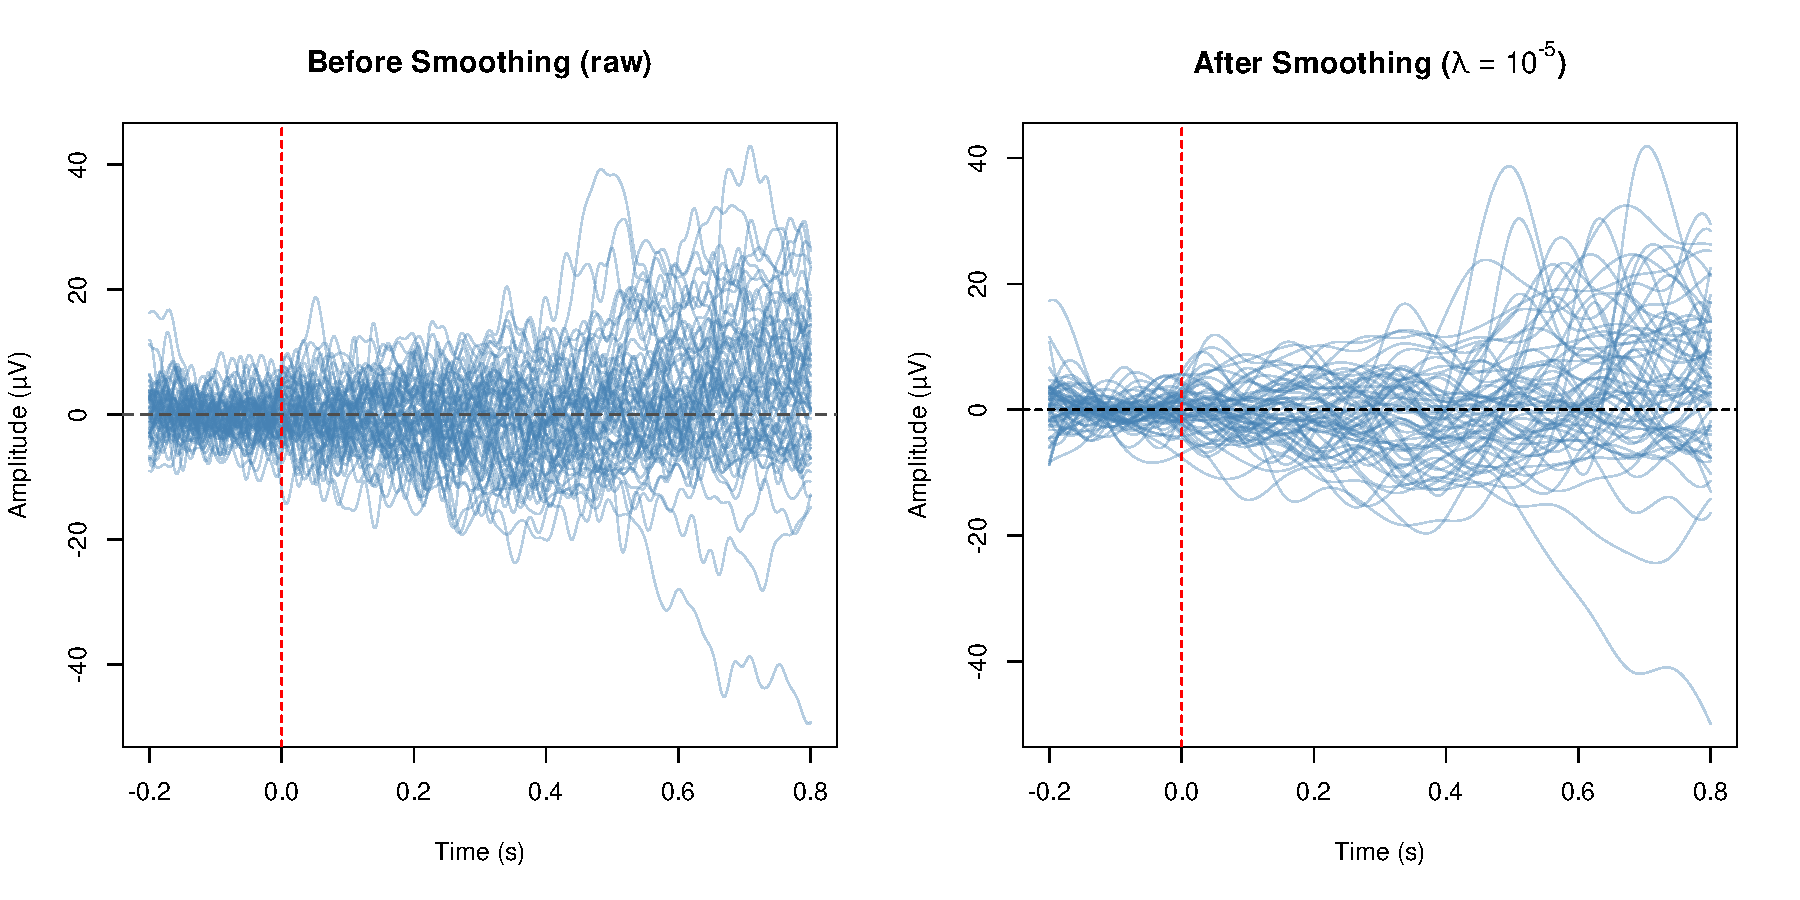
\includegraphics[width=1\textwidth]{02_before_after_smoothing.pdf}

\end{frame}


\section{Exploratory Data Analysis}

\begin{frame}{Mean and standard deviation}

    \centering
    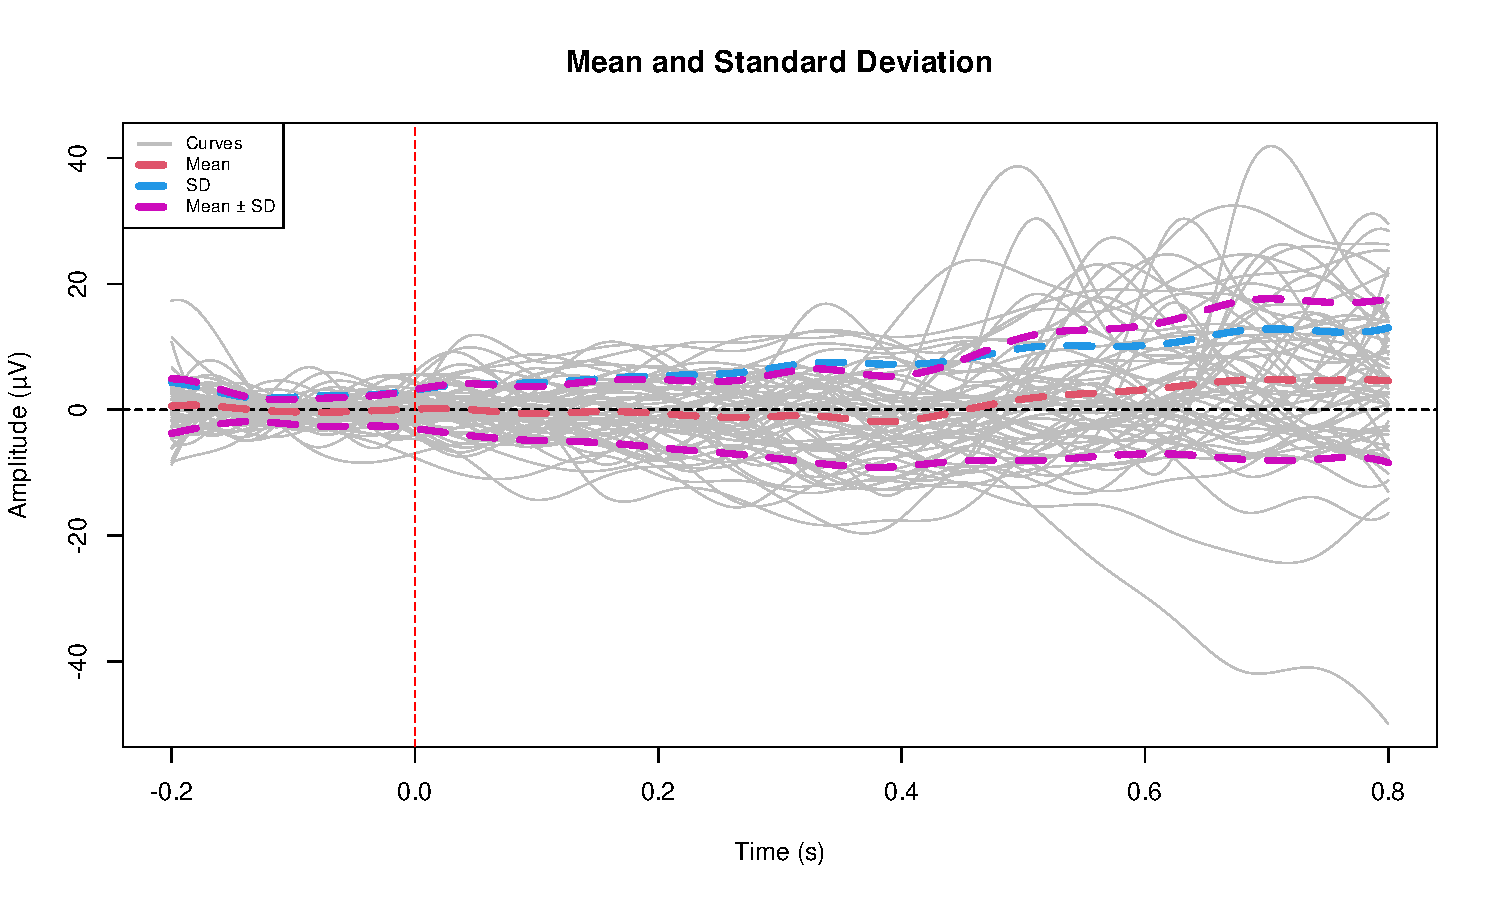
\includegraphics[width=1\textwidth]{04_mean_sd.pdf}

\end{frame}


\begin{frame}{Covariance}
    \begin{columns}
        \begin{column}{0.5\textwidth}
            \centering
            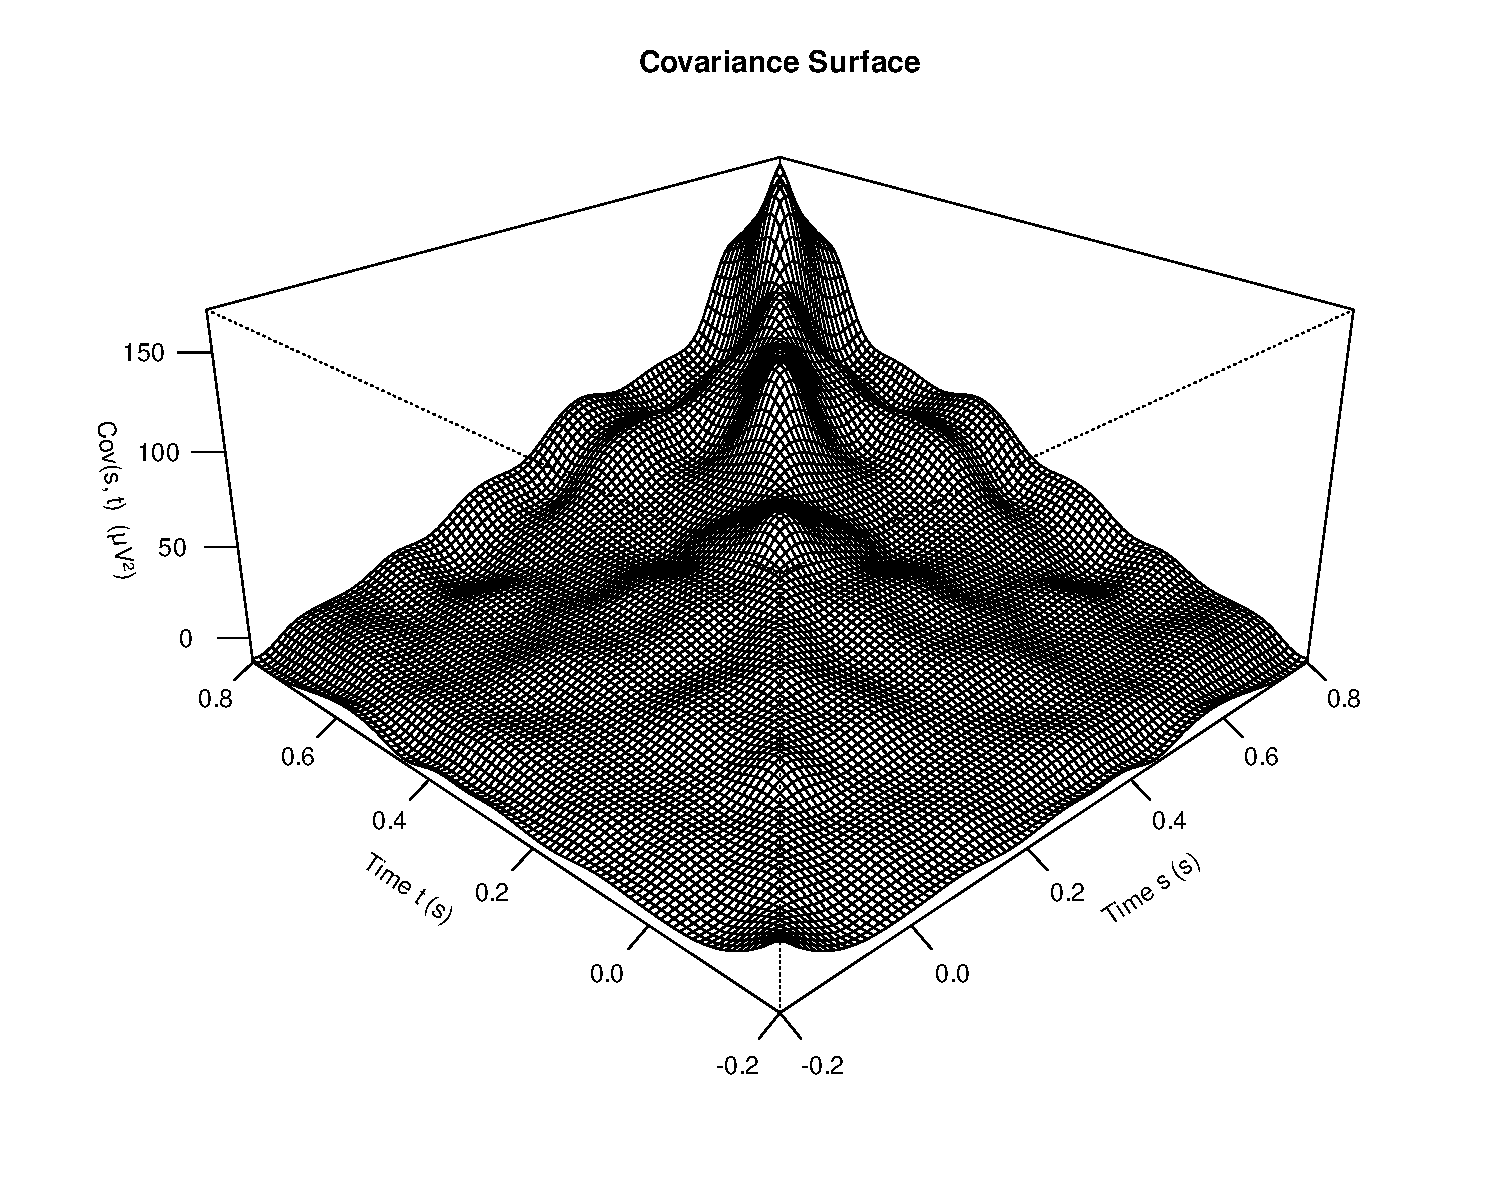
\includegraphics[width=\textwidth]{05_covariance_persp.pdf}
        \end{column}
        \begin{column}{0.5\textwidth}
            \centering
            
\includegraphics[width=\textwidth]{07_covariance_image.pdf}
        \end{column}
    \end{columns}
\end{frame}





\begin{frame}{Principal Component Analysis I}

    \centering
    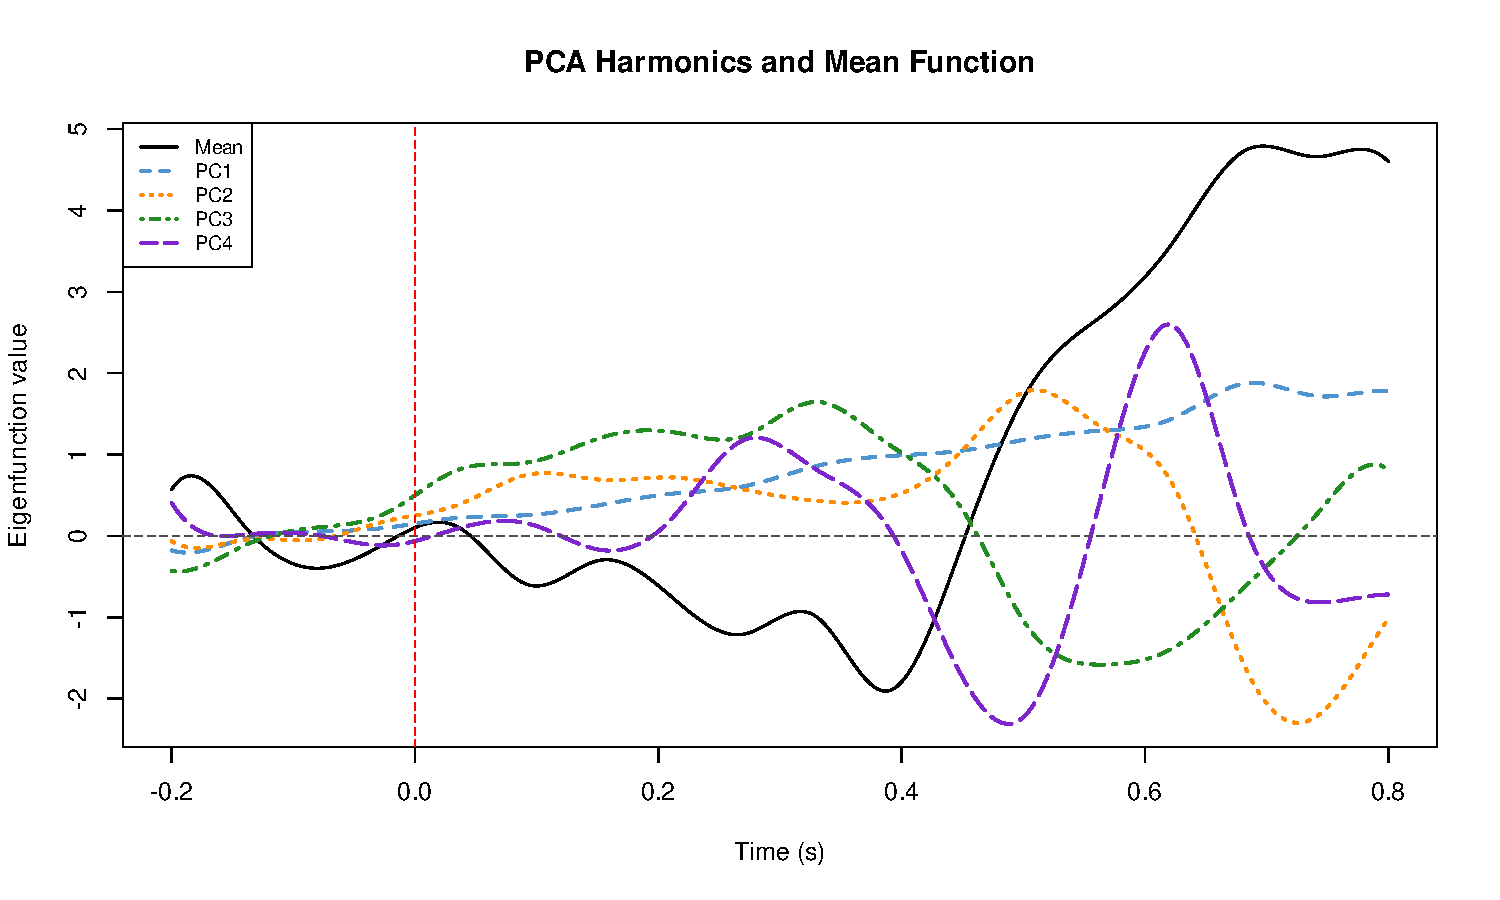
\includegraphics[width=1\textwidth]{13_pca_harmonics.pdf}

\end{frame}



\begin{frame}{Principal Component Analysis II}

    \centering
    
\includegraphics[width=1\textwidth]{15_pca_perturbation.pdf}

\end{frame}



\begin{frame}{Functional Box Plot}
    \centering
    
\includegraphics[width=1\textwidth]{21_fbplot_MBD.pdf}

\end{frame}



\begin{frame}{Outliers}

    \centering
    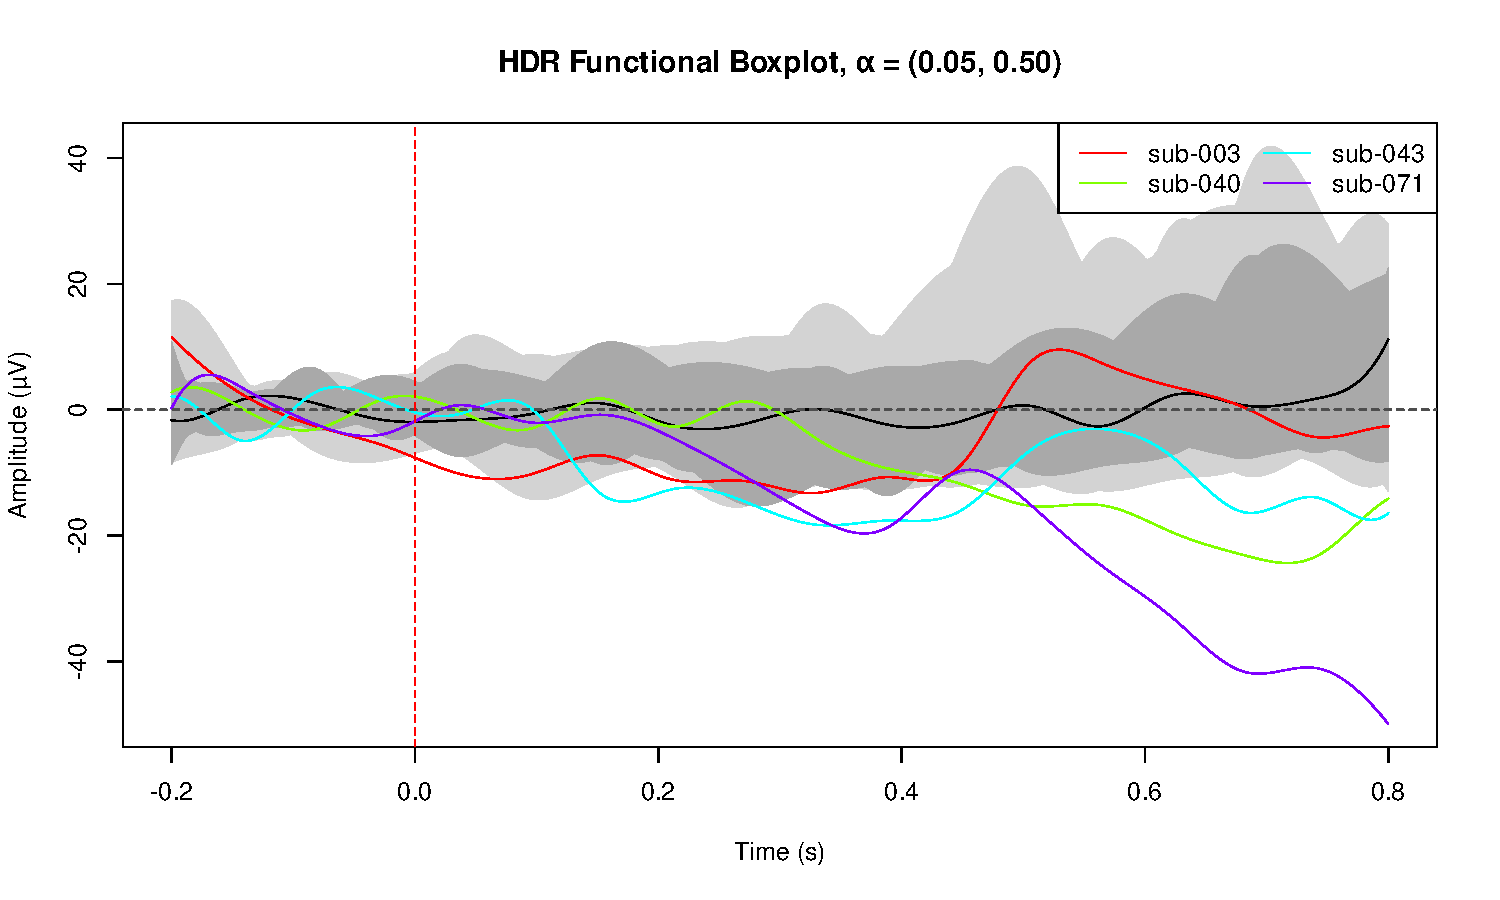
\includegraphics[width=1\textwidth]{32_hdr_functional_005.pdf}

\end{frame}




\section*{Acknowledgements}
\begin{frame}
\textcolor{myNewColorA}{\Huge{\centerline{Thank you for your time!}}}

\end{frame}




\end{document}

